\section{Mini-projet d'e-banking}

À la suite de notre formation, nous avons mis en pratique nos connaissances dans un mini-projet de réalisation d'une application web d'e-banking : MF-Bank.\\

Le code source de notre projet ce trouve à l'adresse suivante : \url{https://github.com/excilys-pdalpra/excilys-mfb}.

Une version de l'application est disponible publiquement sur le PaaS Jelastic\cite{jelastic} : \url{ http://mfbanking.j.layershift.co.uk/}. Les identifiants utilisables sont :

\begin{itemize}
	\item Utilisateur : login : \textit{user} / pswd : \textit{user}
	\item Administrateur : login : \textit{admin} / pswd : \textit{admin}
\end{itemize}

\subsection{Cahier des charges}

L'application à réaliser est une application web de gestion des comptes. Les fonctionnalités sont les suivantes :

\begin{itemize}
	\item S'identifier,
	\item Consulter la liste de ses comptes,
	\item Consulter le détail des opérations pour un compte et un mois donné,
	\item Consulter le détail des opérations cartes pour un compte et un mois donné,
	\item Effectuer un virement entre ses comptes,
	\item Consulter l'historique de ses virements,
	\item Exporter au format Excel le relevé des opérations pour un mois donné.
	\item Exposer ces fonctionnalités sous la forme de web services.
\end{itemize}

\subsection{Méthodologie}

\subsubsection{Gestion du projet}

Étant cinq stagiaires à être arrivés le même jour et un autre la semaine suivante, nous avons formé une équipe de six personnes pour réaliser ce projet. Il nous avait été laissé la possibilité de former deux groupes projet de trois personnes, mais nous avons préférer former une seule équipe et ainsi avoir la possibilité d'approfondir de façon plus importante le projet.\\

La méthode que nous avons utilisé pour gérer ce projet a été un mélange entre la méthode Scrum et l'XP, soit deux méthodes Agiles. L'utilisation des méthodes Agiles repose en grande partie sur le constat qu'un produit logiciel voit la plupart du temps ses demandes en fonctionnalités évoluer au fur et à mesure, et que cela est très difficile à prendre en compte avec un  système non itératif, comme pas exemple le cycle en V. Ici, le but est d'effectuer de courtes itérations d'une à deux semaines au bout desquelles un produit utilisable est livré. Dans notre cas, du fait de la durée du projet, nous avons fait des itérations (ou sprints) d'une semaine.\\

La première itération, appelé Sprint 0 a consisté en la mise en place de l'environnement de développement, de l'environnement d'intégration ainsi que des conventions à utiliser. C'est au cours de cette semaine que nous avons aussi choisi le socle de technologies que nous utiliserions. Nous avons aussi réfléchi à l'architecture générale de l'application. Tous ces choix sont expliqué dans la suite du rapport. À la fin de ce premier Sprint, nous avons fait une réunion avec Stéphane LANDELLE, le directeur technique d'\ebi{}, pour valider nos choix.\\

Les autres itérations ce sont ensuite déroulées de la façon suivante :
\begin{enumerate}
	\item Réunion avec le \flqq{}product owner\frqq{} (client dans le vocabulaire Scrum), c'est à dire Stéphane LANDELLE, pour sélectionner les fonctionnalités à développer dans cette itération,
	
	\item Développement des fonctionnalités, principalement en pair programming pour mutualiser les connaissances,
	
	\item Réunion technique avec Stéphane LANDELLE en tant que référent technique pour auditer notre code,
	
	\item Remaniement (refactoring) du code suite aux remarques.
	
	\item Réunion avec le \flqq{}product owner\frqq{} pour présenter les fonctionnalités implémentées.\\
\end{enumerate}

De plus, chaque jour nous réalisions un \flqq{}daily Scrum\frqq{} à heure fixe : c'est une courte réunion dans laquelle tout les intervenants sont debout, pour pousser à la concision, et répondent à trois questions :
\begin{enumerate}
	\item Qu'est-ce que j'ai fait hier ?
	
	\item Qu'est-ce que je compte faire aujourd'hui ?
	
	\item Quelles sont les difficultés que je rencontre ?\\
\end{enumerate}

Cette méthode permet d'avoir un résultat chaque semaine à montrer au client. Le client peut donc voir l'évolution du projet en temps réel, tester les parties déjà développées ce qui permet d'avoir un retour rapide. De plus, le client est beaucoup plus investi dans le projet et peut facilement ajuster ou modifier le cahier des charges.\\

Pour le développeur, les itérations permettent de ne pas avoir un travail trop répétitif puisque dans chaque itération, on retrouve toutes les phases du cycle en V classique. Il n'y a donc plus de grandes phases de développement, de tests, de recette, \dots{}

La méthode Scrum impose également définir les conditions pour considérer qu'une tâche est terminée (Definition de \og Fini Fini \fg{}). Dans le cadre de l'application d'e-banking, notre définition de \textit{Fini Fini} était la suivante :
\begin{itemize}
	\item Développé
	\item Testé (en local et sur le serveur d'intégration)
	\item Refactoré
	\item Revu par un pair
	\item Documenté (Javadoc)
\end{itemize}

\subsubsection{Intégration Continue}

Nous avons aussi mis en place une autre pratique Agile : l'intégration continue. C'est un processus de développement issu de la méthode XP. Ceci permet de répondre à un des principes de cette méthode : la capacité de fournir à tout moment une version fonctionnelle de l'application au client.

L'intégration continue repose sur quelques grands principes :
\begin{itemize}
	\item Utiliser un logiciel de contrôle de versions
	\item Automatiser le processus de build
	\item La build doit être \og auto-testante \fg{} : Les tests doivent être automatiquement exécutés après la compilation.
	\item La compilation doit rester courte, et ainsi pouvoir builder le projet régulièrement.
	\item Le résultat de la build doit être visible par tout le monde et les livrables produits facilement accessibles\\
\end{itemize}


\subsubsection{Build incassable}

Enfin dans le but d'automatiser un peu plus notre processus d'intégration continue nous avons mise en place une build incassable, dont le principe est le suivant : conserver en permanence le \textit{trunk} (la branche principale) exempt de bugs, en interdisant aux développeurs de mettre directement à jour celui-ci. Cette tache est laissée au serveur d'intégration continue qui réalise la mise à jour uniquement si le build réussi.\\

Le fonctionnement est le suivant :\\
\begin{figure}
	\centering
		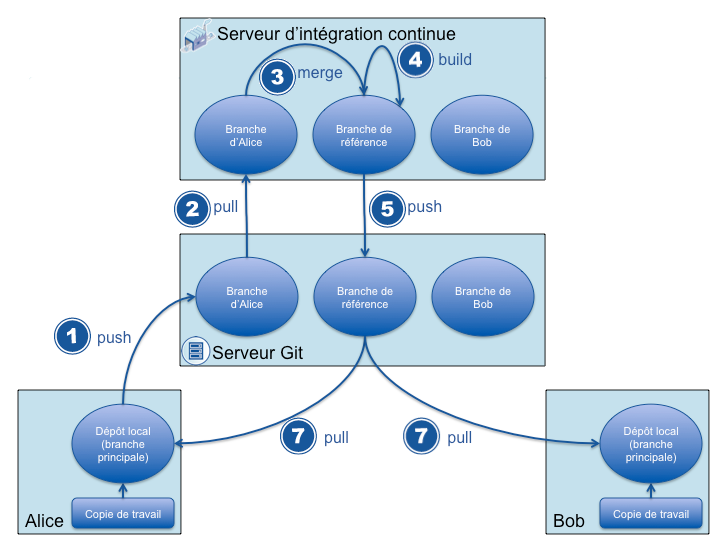
\includegraphics[scale=0.5]{images/build_incassable.pdf}
	\caption{Worflow dans un système de build incassable}
\end{figure}

\begin{enumerate}
	\item Chaque développeur dispose d'une \textit{branche}, une version parallèle des sources du dépôt. Quand des modification ont été effectuées et doivent être synchronisées avec le \textit{trunk}, le développeur \textit{push} ses modifications sur sa branche.
	\item Le serveur d'intégration continue détecte les modifications apportées sur la branche du développeur, et récupère ses modifications
	\item	Le serveur d'intégration fusionne alors ces modifications avec sa copie locale du \textit{trunk}
	\item Une build est alors tentée, afin de vérifier que le code compile bien et que l'ensemble des tests passent\ldots
	\item Si la build réussit, le serveur d'intégration propage alors les modification sur le trunk
	\item Les développeurs peuvent alors se synchroniser avec le \textit{trunk}, en étant assuré que l'ensemble est parfaitement fonctionnel
\end{enumerate}
L'inconvénient de la build incassable est qu'elle repose sur le respect de bonnes pratiques de codage de la part des développeurs, notamment l'écriture de tests exhaustifs.\\
En effet, sans une couverture de test adéquat, du code fonctionnement faux peut se retrouver dans la branche principale, pourtant censée ne contenir que du code sûr sur lequel les autres développeurs peuvent s'appuyer sans crainte.  

La procédure que nous avons suivi pour mettre en place ce dispositif est détaillée sur le blog du cabinet d'expertise informatique Octo\cite{build}.

\subsection{Choix techniques}

Le choix des technologies à utiliser était en grande partie libre, même s'il était soumis à l'approbation de Stéphane. Voici les technologies que nous avons choisi d'utiliser et nos motivations :

\subsubsection{Gestionnaire de version}

Il permet de travailler sur un projet de manière collaborative et simultanée. Il existe principalement deux gestionnaires de version : Git et Subversion, dont la philosophie diffère.\\

Subversion est le plus répandu actuellement car plus ancien. C'est un système de versionnement centralisé, i.e. qu'il n'existe qu'un seul dépôt des versions, robuste qui à fait ses preuves. Le développement est fortement linéaire, car la création d'une branche demande la copie complète du code.

Git est lui plus récent (2005). Il a été créé par Linus Torvalds pour gérer le développement du noyaux Linux. C'est un système de versionnement décentralisé, chaque utilisateur dispose d'un dépôt local, très puissant. Il tire profit au maximum des branches pour avoir des fonctionnalités se développant en parallèle sans rentrer en conflit. Une fois une fonctionnalité développée sa branche est fusionnée à la branche principale généralement appelée master.\\

Nous avons choisi d'utiliser Git, car même si ce n'est pas actuellement le système le plus utilisé, la puissance et la flexibilité qu'il apporte en feront surement le leader dans un futur proche. De plus l'utilisation de cette outil nous a permis de mettre en place un processus d'intégration continue très intéressant qui sera détaillé ci-après. Malgré son coté décentralisé nous avions besoin d'un dépôt distant permettant de centraliser le travail et d'accéder au code de n'importe où. Nous avons ainsi choisi d'héberger notre projet sur GitHub, plateforme d'hébergement de projet open-source utilisant Git. 

\subsubsection{Construction du projet}

Plusieurs systèmes permettent de construire des projets Ant, Maven, Gradle, \dots{} Ant est le plus ancien. C'est globalement un outil qui permet d'écrire des scripts pour construire des applications. Il est très apprécié car il est très flexible.\\

Maven est plus récent, s'appuie sur des script de build en XML, et se base sur le principe de \flqq{}convention over configuration\frqq{}, c'est à dire qu'il encourage le développeur à respecter certaines conventions pour faciliter la construction du projet comme par exemple l'arborescence du projet, i.e. emplacement des sources, des sources de test \dots{}. Il inclut aussi un système de gestion de dépendance qui va directement chercher les librairies externes dans des dépôts Maven accessibles publiquement.\\

Gradle quant à lui est le plus récent. Il reprend beaucoup des principes de Maven, notamment la gestion des dépendances et le principe de \flqq{}convention over configuration\frqq{}, mais permet aussi une plus grande flexibilité se rapprochant ainsi plus de Ant, grâce à des script écrit en Groovy.\\

Nous avons choisi Maven car c'est actuellement le plus utilisé en entreprise et qu'il est pour des projets relativement classique le plus abouti.

\subsubsection{Système de Gestion de Base de Données (SGBD)}

Afin de persister nos données nous avons besoin d'un SGBD. Il existe de nombreuses possibilités et l'application à réaliser n'a pas besoin de fonctionnalités avancées hormis une gestion des transactions pour garantir la cohérence de nos tables.\\

Les deux principaux SGBD open source sont MySQL et PostgreSQL. Ces deux solutions sont assez proches. Nous avons choisi PostgreSQL pour son plus grand respect de la norme SQL.

\subsubsection{ORM}

Le choix de d'Hibernate comme ORM nous a été imposé. En effet il est actuellement le standard de facto et sa maitrise est un impératif de notre métier. Nous avons par contre choisi d'utiliser la version 4, qui est une implémentation de la spécification JPA. Il est a noter que l'implémentation de référence de cette spécification est TopLink, mais qu'elle est beaucoup moins utilisée. 

\subsubsection{Conteneur d'application}

Les conteneurs d'applications sont des boites à outils fournissant des services pour résoudre des problématiques que toute application rencontre. Dans le monde Java, il en existe principalement deux : JEE et Spring.\\

A nouveau le choix de Spring nous a été imposé. Car même si il n'est pas porté par un standard Spring est le conteneur le plus répandu dans le monde de l'entreprise. Spring est un conteneur léger qui ne nécessite pas un serveur d'application mais un simple conteneur de Servlet contrairement au conteneur JEE. Ceci permet d'éviter, au moins pour le développement de l'application, la complexité, la lenteur et la lourdeur de serveur comme JBoss, Weblogic ou Websphere et de simplement déployer son application dans un Tomcat ou un Jetty qui sont beaucoup plus rapide.\\

De plus, nous avons aussi utiliser Spring pour l'intégration d'Hibernate (Spring-DB), la gestion des transactions (Spring-TX), le framework MVC (Spring-MVC), la sécurité (Spring-Security) et la mise en place de traitement batch (Spring-Batch). 

\subsubsection{Serveur}

Puisque nous utilisons Spring, nous pouvons utiliser un simple conteneur de Servlet. Il en existe principalement deux Jetty et Apache Tomcat. Nous avons préféré Tomcat car encore une fois, il est le plus répandu et que sa robustesse n'est plus a démontrer. Il sert entre autre de conteneur de Servlet dans le serveur JBoss et sert par exemple en production chez Atos Worldline. 

\subsubsection{Frameworks de tests}

Les tests sont une composante importante d'un projet informatique. Il existe différents types de tests qui répondent à différentes problématique.

Tout d'abord les tests unitaires qui vont permettre de s'assurer du bon fonctionnement et de la non régression d'un composant logiciel. Dans ce but nous avons utilisé JUnit, qui est le standard de facto dans le monde Java. D'autre alternative existe comme TestNG qui d'un point de vue strictement technique est plus performant. Mais la prédominance de JUnit dans le monde professionnel nous a fait préférer cette solution.\\

Pour pouvoir isoler les composants logiciel lors des tests unitaires nous avons aussi utilisé un framework de mock. Mocker un objet consiste à remplacer un objet par un faux dont on fixe le comportement. Si par exemple une classe A utilise une autre classe B pour son fonctionnement. Lorqu'on veut tester uniquement la classe A, il faut mocker la classe B et injecter le mock dans la classe A. Ainsi les bugs dans la classe B n'interfèrent pas avec les tests de la classe A. Pour cela nous avons utilisé Mockito qui nous a été recommandé par Stéphane. Les autres possibilités sont EasyMock ou PowerMock. L'avantage de Mockito par rapport à Easymock est que nous ne sommes pas obligé de spécifier de façon exhaustive le comportement du mock.\\

Ensuite il existe les tests d'intégration qui vont permettre de tester fonctionnellement l'application et ainsi s'assurer du bon comportement général. Notre choix s'est porté sur Selenium. Ce framework permet de jouer des actions utilisateurs comme des clics sur un bouton, le remplissage de formulaires, et de spécifier un certain nombre de contrôles pour vérifier le bon comportement.

Enfin nous avons aussi réalisé des tests de monté en charge grâce à Gatling. C'est tests visent à s'assurer du bon fonctionnement de l'application lorsque celle-ci est utilisée en simultané par une population d'utilisateur.

\subsubsection{Serveur d'intégration}

Un serveur d'intégration est un serveur qui périodiquement récupère le code source d'un projet depuis un gestionnaire de version, le construit, exécute les tests unitaires et les tests d'intégrations et génère un rapport avec le résultat de la construction du projet et de l'exécution des tests. Ce serveur permet d'avoir un système d'intégration continue : lorsqu'un développeur modifie le code source et envoie ses modifications au gestionnaire de version, le serveur d'intégration va permettre de vérifier qu'il n'y ait pas de régression et garantir le bon fonctionnement de l'application.\\

Nous avons choisi d'utiliser Jenkins (anciennement Hudson) car c'est le serveur d'intégration open source le plus utilisé dans le monde Java. Il est entre autre la pierre angulaire du PaaS (Platform as a Service) de CloudBees DEV@Cloud.

\subsubsection{Framework de web services}

Les web services sont des services distribués utilisant HTTP comme protocole de transport. Ces web services permettent à une application tierce d'interagir avec notre application. Il existe principalement deux types de web services : SOAP (Simple Object Access Protocol) et REST (REpresentational State Transfer).\\

SOAP est un standard qui s'appuie principalement sur XML ce qui fait de lui un protocole très verbeux et est généralement utilisé dans un même réseau, c'est à dire entre des applications d'un même système d'information par exemple.\\

REST n'est pas à proprement parlé un protocole mais simplement un type d'architecture : puisqu'on utilise HTTP pour le transport, utilisons toutes les possibilités de ce protocole. Il est généralement utilisé en combinaison avec JSON (JavaScript Object Notation) permettant de représenter les objets sous la forme de chaîne de caractères.\\

Pour la mise en place des web services nous avons choisi Apache CXF puisqu'il permet de faire des web services SOAP et REST en implémentant les respectivement les spécification JaxWS et JaxRS et s'intègre complètement avec Spring.

Ces technologies ont été choisies principalement car elles sont très répandues dans le monde de l'entreprise. Ce mini-projet nous a donc permis de nous faire la main sur les technologies que nous sommes le plus à même de rencontrer en clientèle.

\subsection{Architecture du projet}

L'architecture de MF Banking repose sur le modèle de l'architecture $N$-tiers.
Le principe de cette architecture consiste à découper l'application en plusieurs couches (le plus souvent trois couches), chacune ayant un but très précis. Ce découpage présente deux avantages majeurs :

\begin{itemize}
	\item chaque couche ayant un but bien précis, celle-ci est plus facile à maintenir. De plus le couplage des différents composants est relativement lâche. 
	\item Le faible couplage permet aux différentes couches d'\^{e}tre interchangeables.
\end{itemize}

Il en résulte une application hautement modulaire, où chaque couche peut dans la théorie être remplacée ou mise à jour en ayant un impact réduit sur le reste de l'application.\\

Dans le cas d'une architecture 3-tiers, que nous avons utilisé pour MF Banking, les  couches sont les suivantes :

\begin{figure} [h!]
	\centering
		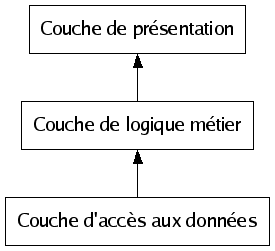
\includegraphics[scale=0.5]{images/ntiers.pdf}
	\caption{Architecture 3-tiers}
\end{figure}

Le rôle de la couche d'accès aux données est, comme son nom l'indique, d'accès aux données de l'application. Typiquement, cette couche se charge d'accéder à une base de données et d'y récupérer les informations ou d'en stocker des nouvelles.\\
 
La couche de logique métier est le pivot de l'application : c'est dans cette couche qu'est gérée toute la logique propre au métier de l'application que l'on souhaite développer, et sert donc de pont entre les données et la façon dont elles sont présentées à l'utilisateur.\\

Enfin, la couche de présentation est celle qui est en charge d'afficher les données de l'application.\\
 
Les Web Services que nous avons mis en place s'appuient sur la couche métier et viennent exposer une partie du métier à l'extérieur.\\
 
Les frameworks permettant l'injection de dépendances tels que Spring simplifient grandement la mise en place d'architecture n-tiers.\\
En effet la possibilité de spécifier les dépendances d'une instance de classe seulement à l'exécution permet de réellement programmer en ne manipulant que des interfaces. On peut ainsi assembler facilement les différentes couches, garantir un minimum de couplage et obtenir une grande modularité de l'application. 
 
\subsubsection{Schéma de la base de données}
	\begin{figure}[h!]
		\centering
			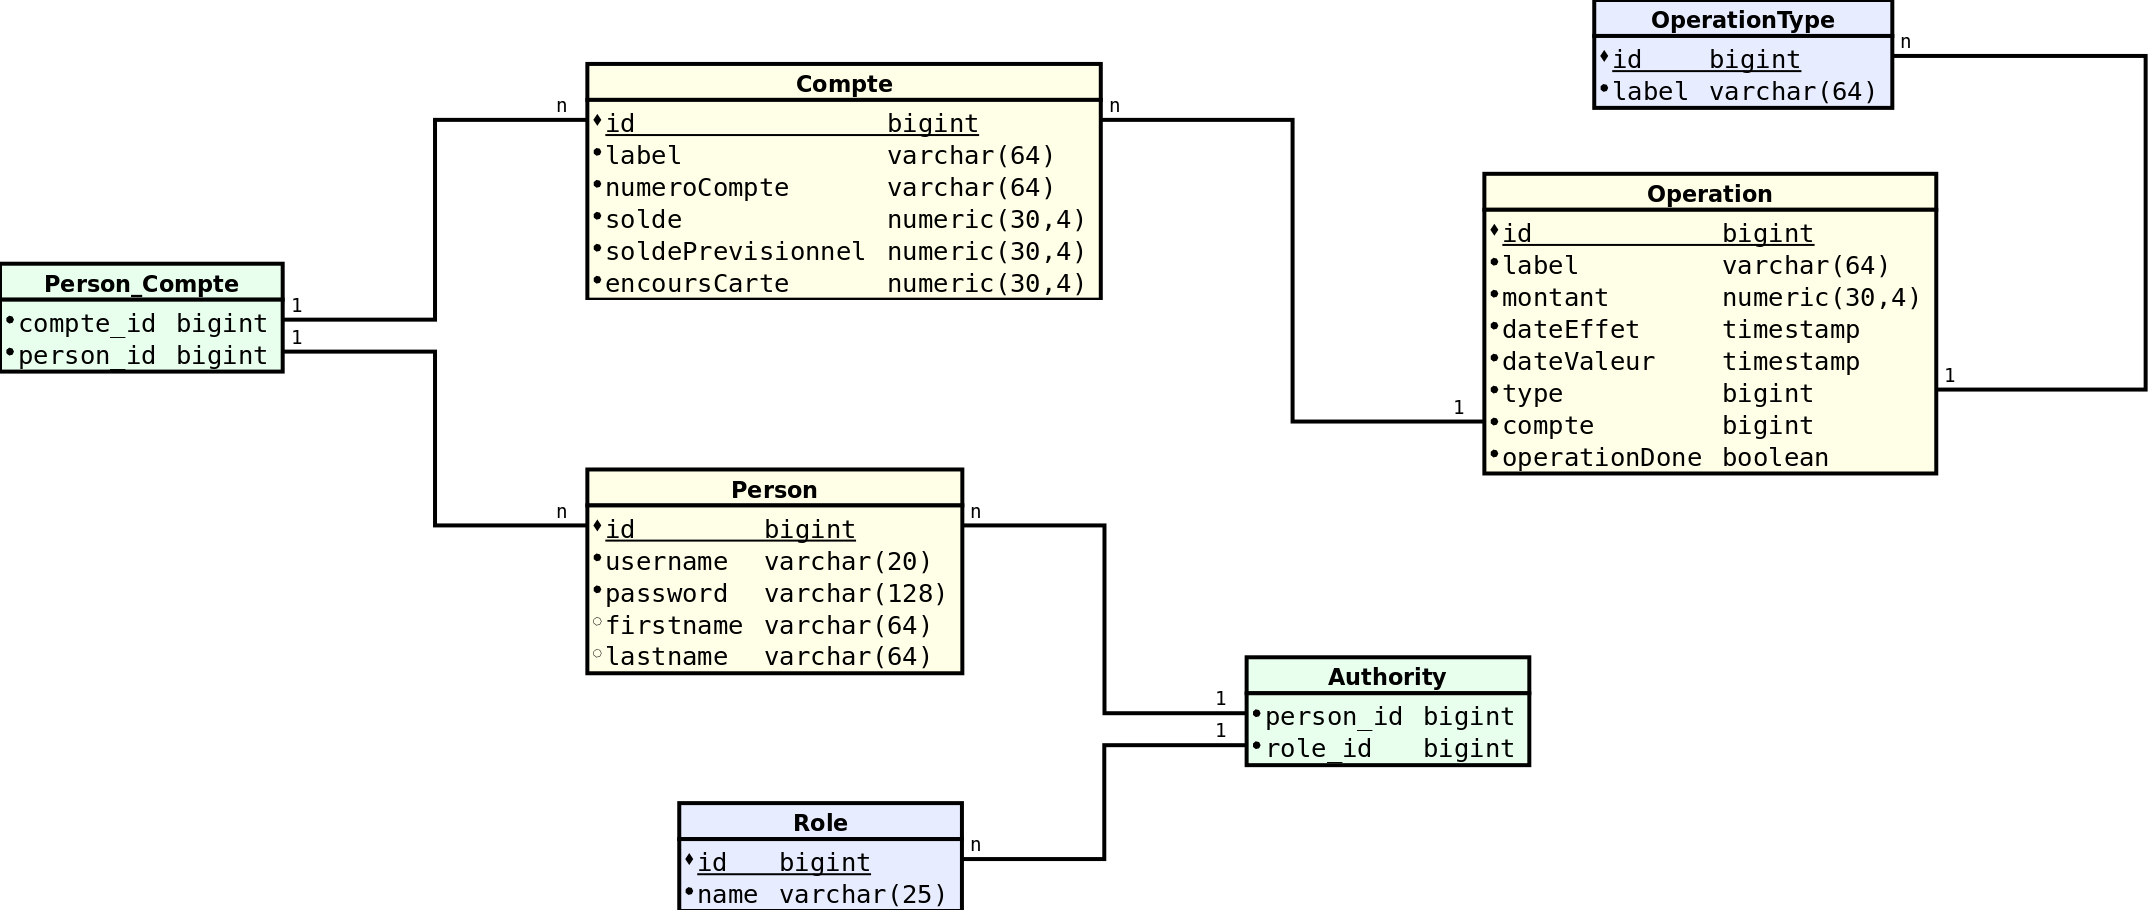
\includegraphics[scale=0.25]{images/diagramme_modele.pdf} 
		\caption{Modèle E/A de la base de données}
	\end{figure}

Lexique des différentes tables :
\begin{itemize}
	\item Person : liste des clients de MF Banking
	\item Role : liste des rôles des utilisateurs (client ou administrateur)
	\item Authority : table de jointure entre Person et Role. Ceci était nécessaire car un utilisateur pouvait être à la fois client et administrateur  
	\item Compte : liste des comptes des utilisateurs
	\item Operation : liste des opérations bancaires effectuées sur les comptes
	\item OperationType : liste des types d'opérations bancaires (chèque, carte bleue, virement et espèce)
\end{itemize}

\subsubsection{Structure}
Par le biais de Maven, nous avons découpé notre application en plusieurs modules qui suivent l'architecture n-tiers décrite ci-dessus avec une granularité plus fine :

\begin{itemize}
	\item Entities
	\item DAO
	\item Services et Services API
	\item Batch
	\item Web
	\item Webservices
	\item Application Android
\end{itemize}

\subsubsection*{module Entities}

Ce module regroupe les différentes entités de notre application, miroir objet de notre base de données ainsi que les scripts Liquibase de mise à jour du schéma de base de données.\\
La librairie Liquibase nous a permis de construire notre schéma de base de données de manière incrémentale  au fil des réalisations de user stories.\\

\subsubsection*{module DAO}

Le module DAO correspond à la couche d'accès aux données.\\
DAO est l'acronyme de \textit{Data Access Object} : un DAO est une objet dont le but est d'accéder et de modifier les données stockées par l'application.\\ 
Sont centralisés dans ce module l'ensemble de la configuration Spring ayant trait à l'accès aux bases de données (connexion, infrastructure Hibernate/JPA, gestion des transactions\ldots) ainsi que le code en charge de la récupération des données depuis la base de données, en se basant sur les entités définies dans le module Entities.\\

En production, l'application utilisait une base de données PostgresSQL mais une base de données H2 a été également utilisée pour effectuer des tests unitaires.Cette base, comme les bases Derby et HSQLDB, présente l'avantage de pouvoir fonctionner uniquement en mémoire, ce qui est très adapté dans le cadre de tests unitaires : la base de données est crée, initialisée grâce à Liquibase et des données sont ajoutées le temps d'effectuer les tests unitaires et la base est détruite une fois le test terminé. On a donc des tests unitaires faciles à reproduire, puisqu'ils sont à chaque fois exécutés sur une base de données vierge.\\

Afin de réaliser les tests unitaires, nous nous sommes aidées d'une librairie développée par Stéphane LANDELLE appelée Spring DB-Unit simplifiant grandement l'insertion de données de tests dans la base en mémoire. 

Idéalement, ce module aurait dû être découpé en deux modules, DAO et DAO API, afin de découpler complètement les interfaces et des DAO et leurs implémentations. En l'état, il est théoriquement possible de faire directement référence aux implémentations, bien que cela n'ait pas été fait.\\
 
\subsubsection*{Services et Services API}

Le module Services est le cœur de l'application, où se situe l'ensemble de la logique métier propre a une application d'e-banking.\\

Afin de respecter au maximum les bonnes pratiques de codage lié à l'architecture $N$-tiers, nous avons testé les services en isolation, sans qu'ils dépendent des implémentations de la couche DAO, grâce à l'utilisation de mocks.\\

\subsubsection*{Batch}

Comme pour une véritable banque, les opérations de MF Banking dispose d'une date d'effet (date à laquelle l'opération a été enregistrée) et d'une date de valeur (date à laquelle l'opération est prise en compte et le solde modifié en conséquence).\\

Cette modélisation impose cependant de mettre à jour automatiquement le solde du compte lorsque la date de valeur d'une ou plusieurs opérations correspond au jour courant.\\
Nous avons mis en place cette mise à jour automatique par le biais d'un traitement batch en utilisant Spring Batch : une tâche de mise à jour du solde est exécutée à intervalles réguliers pour tous les comptes de la banque.\\

\subsubsection*{Web}

Le module Web correspond à la couche de présentation de l'architecture $N$-tiers.\\
Nous avons utilisé le framework Spring MVC pour bâtir notre couche web, car il offrait de nombreux avantages : Spring MVC est parfaitement intégré à Spring et son modèle de programmation est simple et permet de développer rapidement des interactions complexes avec l'utilisateur. Comme son nom le laisse suggérer, Spring MVC tend à se rapprocher d'une architecture Modèle-Vue-Contrôleur.\\

Le module Web est très nettement le module qui a le plus bénéficié de librairies tierces-parties, toujours dans le but de simplifier autant que possible le développement en déléguant les tâches complexes ou répétitives à une librairie.\\
Nous avons utilisé entre autres : 
\begin{itemize}
	\item Bootstrap, développé par Twitter, offre un ensemble cohérent de feuilles de style CSS et de code JS permettant de développer simplement une interface web agréable à utiliser.
	\item Tiles, librairie de \textit{templating} développée par la fondation Apache.
	\item Hibernate Validator est l'implémentation de référence de la Java Validation API.Les fonctionnalités offertes par la JSR-303 nous ont permis de simplifier grandement la validation des formulaires de MF Banking.
	\item POI, API gérant l'écriture de documents Word,Excel et Powerpoint, développé par la fondation Apache.\\
\end{itemize}

Afin de ne pas permettre à un utilisateur anonyme d'accéder aux comptes de n'importe quel client de MF Banking, notre application a été évidemment sécurisée.Une fois de plus, nous avons utilisé une librairie développée par Spring : Spring Security.\\
Spring Security permet de s'abstraire d'une large part de la complexité de la sécurisation d'une application, en ne demandant au développeur que de préciser ce qui doit \^etre sécurisé, les rôles pouvant accéder à une ressource sécurisée et le moyen authentifier un utilisateur.

\subsubsection*{WebServices} 

Le module Webservices permet l'exposition d'une partie de la logique métier de l'application dans le but que celle-ci soit utilisé par des applications tierces.\\  
Nous avons mis en place deux types de Web Services pour MF Banking : des Web Services SOAP et des Web Services REST.\\

Les Web Services SOAP se basent sur l'échange de fichiers XML au format SOAP contenant les informations que les applications doivent se transmettre,en l'occurrence les arguments à passer aux méthodes des Web Services et les valeurs qui sont retournées par ces mêmes méthodes.\\
Les différents services exposés, les types de données acceptés en entrée et retournés sont exposés via un fichier descripteur, au format WSDL (Web Service Definition Language).\\
L'avantage et à la fois l'inconvénient du SOAP est qu'il est basé sur le XML : le WSDL est avant tout un schéma XML et les données fournies au Web Service peuvent être validées grâce au WSDL, évitant ainsi d'envoyer des données incohérentes. Par contre, XML est un format de fichier très verbeux, où la quantité de données \og utiles \fg{} est finalement assez faible à cause des balises XML. \\
L'API Java centré autour de la création de Web Services SOAP se nomme JAX-WS.
Apache CXF,le framework que nous avons utilisé pour gérer les Web Services, propose deux approches pour générer de nouveaux Web Services ou le code y accédant :
 
\begin{itemize}
	\item \textit{code first} : on écrit d'abord le code du Web  Service, et les annotations de JAX-WS fournissent les méta-données nécessaires à la génération du fichier WSDL correspondant à ce Web Service
	\item \textit{contract first} : on écrit d'abord le WSDL et des outils de génération de code se chargent d'écrire le code du Web Service correspondant.\\
\end{itemize}

Nous avons utilisé ces deux approches pour MF Banking :
\begin{itemize}
	\item les Web Services en eux-mêmes étaient \textit{code first}, car nous disposions déjà du code des services (ce qui réduisaient considérablement la quantité de code à écrire) et que l'écriture d'un fichier WSDL s'avérait être une tâche trop complexe à réaliser dans le temps qui nous était imparti.
	\item les WSDL générés ont été réutilisés pour générer le code des clients des Web Services\\
\end{itemize}

Les Web Services REST suivent une approche très différente de celle des Web Services SOAP. L'idée de départ des Web Services REST (REpresentational State Transfer) est de se baser sur les différents \og verbes \fg{} du protocole HTTP pour définir le type d'action réalisée par une méthode d'un Web Service : une requête GET récupère des données, une requête POST ajoute ou met à jour un élément, une requête DELETE supprime un élément\ldots.\\
Contrairement à SOAP, REST n'est pas un standard mais un style de programmation et d'architecture. Il n'y a donc pas de contrainte sur le format des données échangées.\\

\subsubsection*{Application Android}

L'application Android n'était pas une demande explicite du Product Owner, mais celle nous a permis de mettre en oeuvre les Web Services REST que nous avions implémenté.

\begin{figure}[h!]
	\centering
		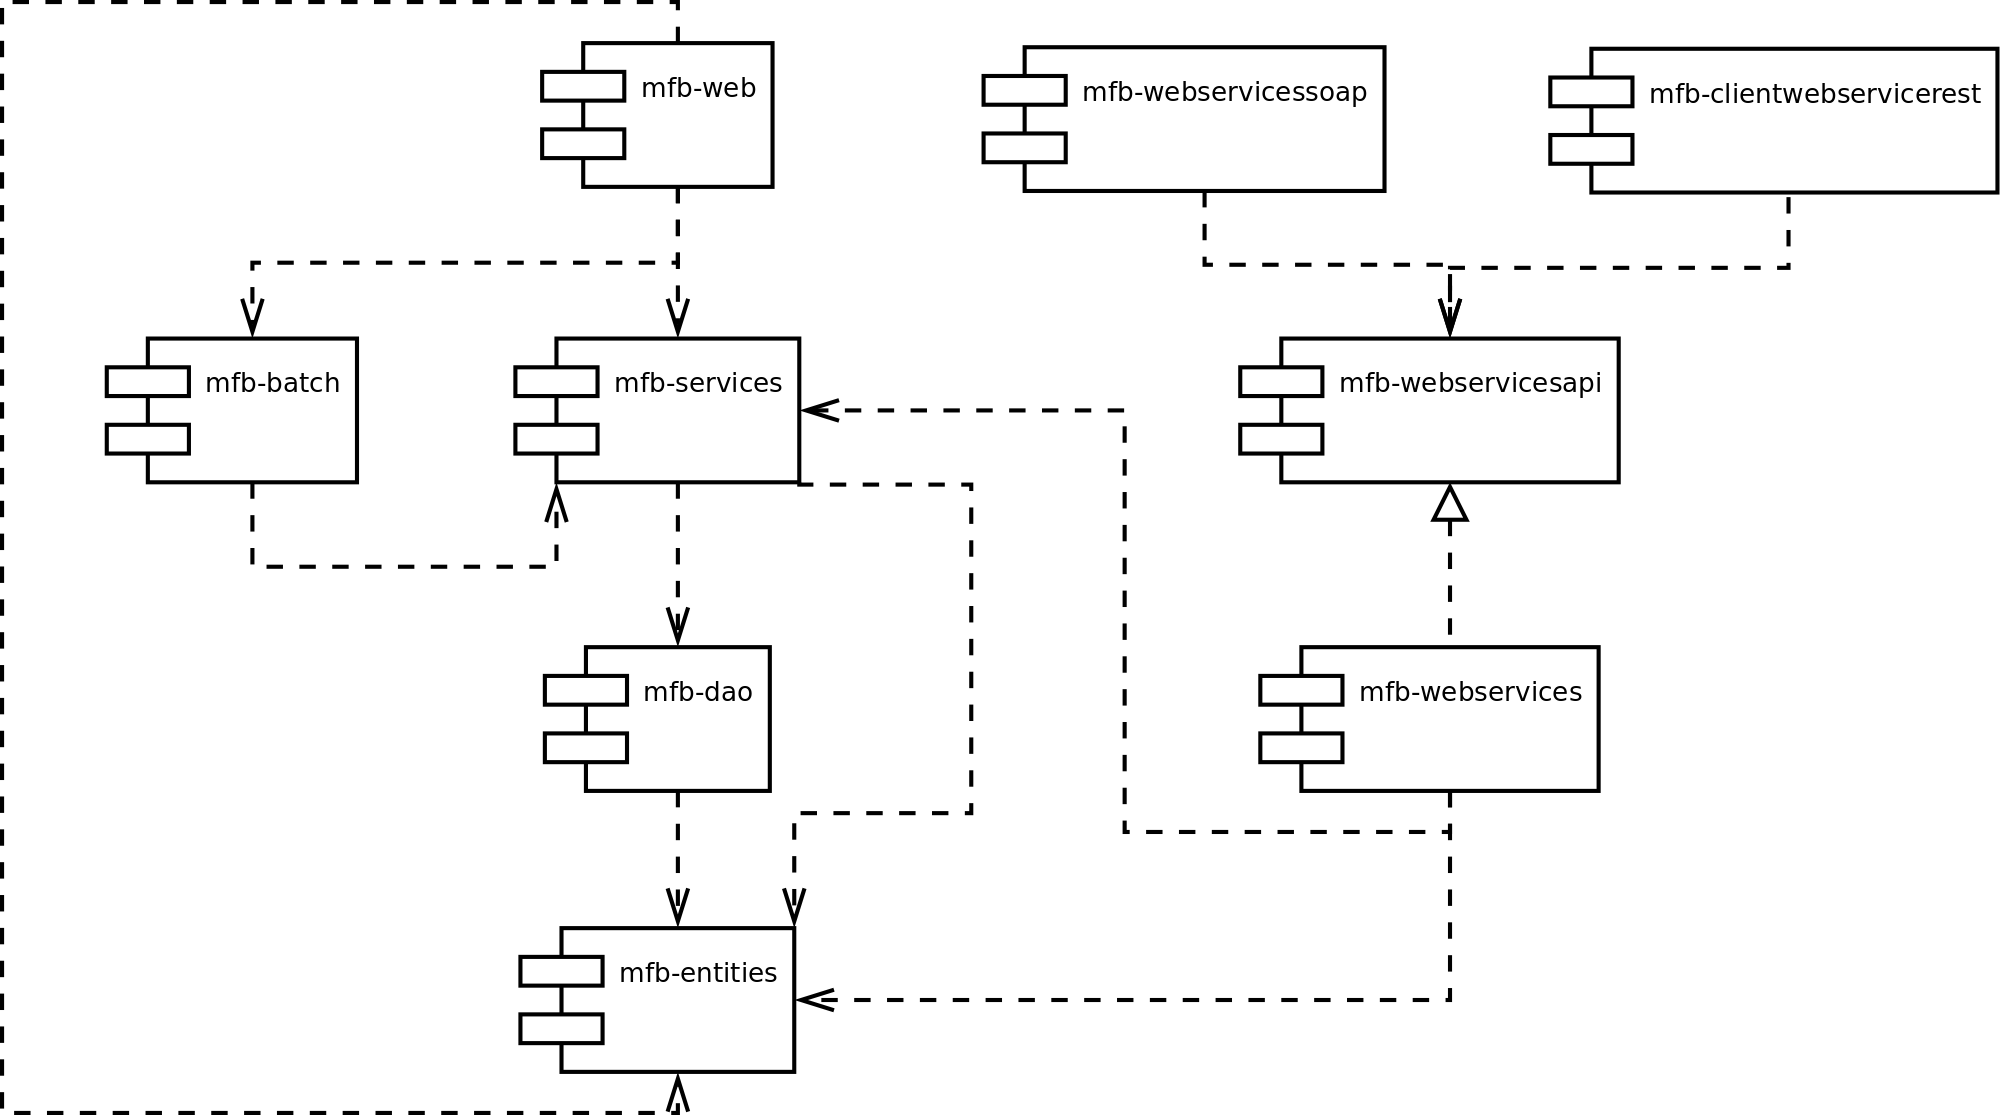
\includegraphics[scale=0.3]{images/diagramme_modules.pdf}
	\caption{Interaction entre les différents modules de MF Banking}
\end{figure}  

\subsection{Organisation des sprints}

\begin{itemize}
	\item Sprint 0 et 1:
	\begin{itemize}
		\item Mise en place de l'environnement de développement : Git, Jenkins, SGBD Postgresql et serveur d'applications Tomcat
		\item Mise en place des conventions de codage (nom des classes et méthodes, formatage du code
		 \item Item 1 : \textit{Consulter sur ma page d’accueil le solde de mes comptes espèce}
		 \item Item 6 : \textit{Accéder à ma page de login}
		 \item Item 7 : \textit{Me logger}
		 \item Mise en place d'une page d'administration basique, pour démontrer le bon fonctionnement du système de rôles 
	\end{itemize}
	\item Sprint 2 :
	\begin{itemize}
		\item Item 2 : \textit{Consulter le détail d'un compte espèce avec le détail des opérations pour un mois donné. Les opérations carte sont cumulées sur une seule ligne}
		\item Item 3 : \textit{Consulter le détail des opérations carte pour un mois donné}
		\item Item 12 : \textit{Accéder au détail des opérations carte par un clic sur la ligne de cumul dans le détail des opérations compte}
	\end{itemize}
	\item Sprint 3 : 
	\begin{itemize}
		\item Item 4 : \textit{Réaliser des virements internes}
		\item Item 5 : \textit{Réaliser des virements externes}
		\item Item 8 : \textit{Exporter au format Excel le relevé des opérations pour un mois donné. Les opérations ne sont pas cumulées.}
		\item Item 9 : \textit{Consulter l'historique de mes virements}
		\item Item 10 : \textit{Consulter sur ma page d'accueil l'encours carte sur chacun de mes comptes espèce}
		\item Item 11 : \textit{Consulter sur ma page d'accueil le solde prévisionnel de chacun de mes comptes espèce}
	\end{itemize}
	\item Sprint 4 :
	\begin{itemize}
		\item Ajout de Web Services REST et SOAP
		\item Amélioration de la zone d'administration : ajout de clients, passage de virements\ldots
		\item Mise à jour automatique du solde, du solde prévisionnel et de l'encours carte
		\item Réalisation de deux applications web et d'une application Android pour tester les Web Services
	\end{itemize}
\end{itemize}

\subsection{Résultat final}

\begin{figure}[H]
	\centering
	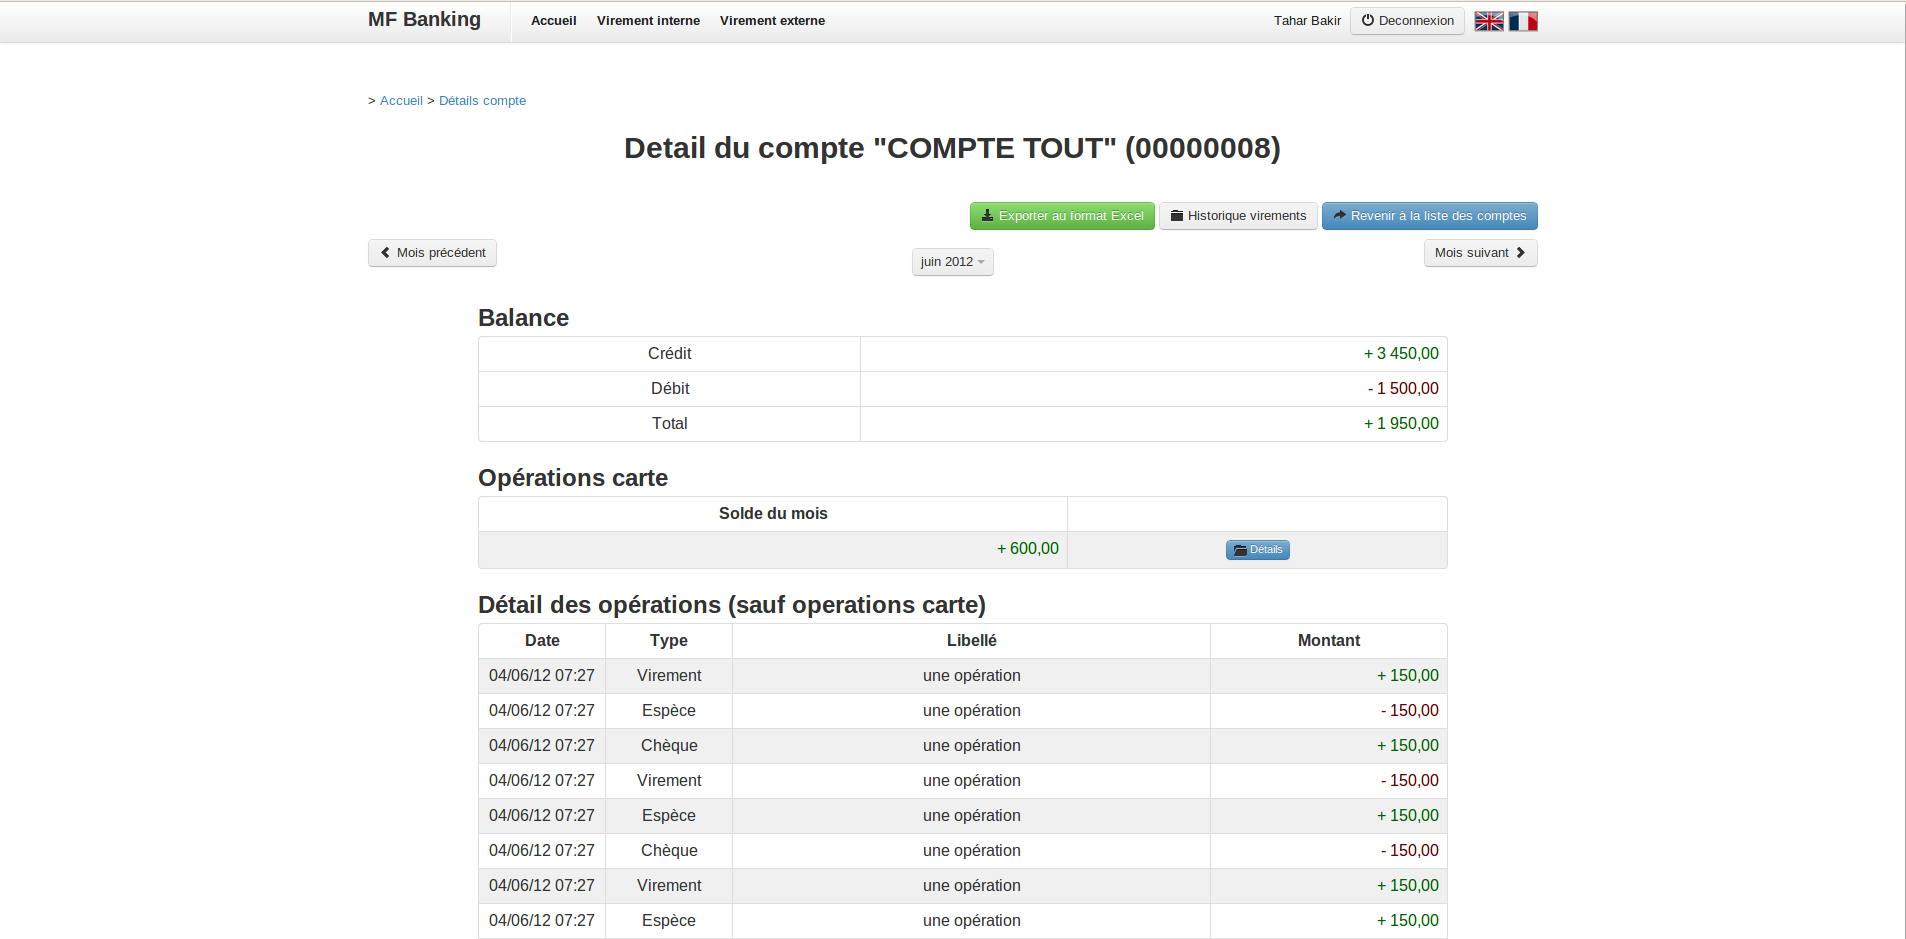
\includegraphics[width=\linewidth]{images/mfb-print-screen.pdf}
	\caption{Résumé du compte pour le mois d'août}
\end{figure}

\subsection{Apport personnel}

Comme tous les autres membres de l'équipe, j'ai participé au développement de la plupart des fonctionnalités de l'application.\\
Les méthodes Agiles prônant la polyvalence des développeurs ma contribution a pris plusieurs formes :
\begin{itemize}
	\item Recherche et prise en main de librairies pour faciliter le développement.
	\item Planification des user-stories.  
	\item Conception du modèle objet et E/A.
	\item Développement des fonctionnalités en binôme.
	\item Réalisation de tests.
	\item Relecture de code.\\
\end{itemize}

J'ai pris part au développement de chacun des modules et ai donc eu l'occasion de travailler sur l'ensemble des technologies mises en œuvre dans MF Banking.\\
 
\subsection*{MF Banking en chiffres}

En résumé, MF Banking, c'est : 
\begin{itemize}
	\item 6 développeurs
	\item 5 semaines de développement
	\item 444 commits
	\item 8000 lignes de code
\end{itemize}

\subsection*{Tests de charge sur MF Banking avec Gatling}

Durant mon travail sur Gatling, et afin de prendre en main cet outil, j'ai été amené à écrire un test de charge de notre application.\\
Ce test de charge, impliquant l'utilisation simultanée de l'application par 1000 utilisateurs, a montré que notre application résistait bien à la charge et qu'elle était donc relativement performante.\\
Ce scénario de test a effectué 110000 requêtes sur MF Banking, donc aucune n'a échoué. Le temps moyen de réponse est de 191 ms, avec un temps de réponse maximal de 9,6 secondes (cf. annexe~\ref{ann:gatling}).\\
Il faut quand même que le scénario de test utilisé n'impliquait pas d'écriture dans la base de données.\\